\chapter{Convolutional Neural Networks}

CNN's are commonly misunderstood to be used just for images, which is false! They are also used for semantic parsing, search query parsing, sentence prediction and more - language tasks! They are obviously popular because of their uses for images though. CNN's can be used for image recognition, classification, and detection. Recognition and detection are different; it's one thing to identify a person as a human and another to know what specific person it is. These neural networks are also used for videos - not just images. If we are trying to track an individual through space and predict where they will be - CNN's can be used.

For now, let's think of ConvNet (CNN) as a black box to which we feed an input, and get an output. To complicate things, we send the output of ConvNet to a feature map (they describe the image in a certain way), and pass it through FC Layers (normal fully connected layers of a neural network).

\textbf{Note (New Terminology - recap of NN):} A perceptron is a node in our neural network that is decided by the product of weights and activations in the previous layer. The input to a node along with the weights for each determine the activation of a certain perceptron. This is then used to compute the perceptrons for the next layer. A fully connected layer is one in which each perceptron in a layer, is connected to all perceptrons in the previous layer.

\section{Architecture}

\href{https://cs231n.github.io/convolutional-networks/#overview}{These notes} by cs231n cover the general architecture (input -> conv -> relu -> pool -> fully connected -> class scores). Look at this after some general reading about CNNs

\section{Convolutions}

A convolution is a mathematical operation on two functions that produces a third function that expresses how the shape of one is modified by the other. Mathematically,

\begin{equation}
    (f * g)[n] = \Sigma_{m= \infty}^{\infty} \; f[m]g[n-m]
\end{equation}

where $n$ is the timestamp. This is slightly hard to understand immediately but signal processing might help understand. This is like a one-dimensional convolution.

The 2D convolution is fairly simple to understand. If we have a kernel - a small matrix of weights. The kernel "slides" over the 2D input data, performing an element wise multiplication with part of the input it is current on, and summing up the results into a single output pixel. Hence, we get a new 2D matrix from our 2D matrix of features.

To see how this works, look at a gif of how convolution works. It is commonly visualized as a matrix tile that is traversing through a larger matrix.

\subsection{Some Uses}

\begin{figure}[h]
    \centering
    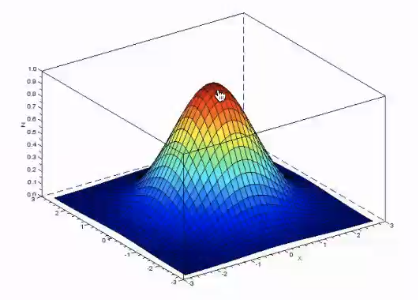
\includegraphics{img/3d-gaussian.png}
    \caption{3D Gaussian}
    \label{fig:my_label}
\end{figure}

Blurring (like blurring an image) can essentially be thought off as taking an average of adjacent pixels. For blurring using convolutional neural networks, we will use an averaging filter that has a gaussian distribution (like the image shown). Here, the central pixel will have the most importance. 

CNN's can also be used for edge detection. For instance, laplacian filter will take a gaussian kernel, and another one, and take the derivative (read more). So these filters help us achieve a lot of things, and convolving a filter with a certain image gives us a response that represents how that portion of the image is represented with respect to our filter.

\section{Techniques}

\subsection{Padding}

Now, if we use a filter and convolute, we get a smaller output matrix. In fact, the corners of the image will never correspond to the center of the filter. This is where padding is generally used. We pad the matrix on the outside with 0's (Zero is usually used) and this lets us get a larger output matrix. Hence, we apply convolutions after padding. The pixels that were previously getting "ignored" because they were at the edge come to focus as they now have neighbouring elements.

\subsection{Striding}

Striding is used to get an output that is smaller than the input.

\subsection{Dilation}

\begin{figure}[hbtp]
    \centering
    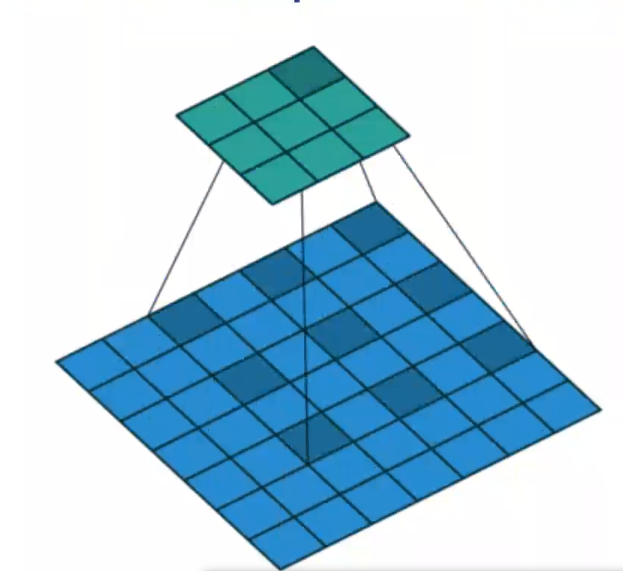
\includegraphics[width=5cm]{img/dilation-cnn.png}
    \caption{Dilation}
    \label{fig:dilation}
\end{figure}

In dilation, we don't choose adjacent elements from our input matrix - but leave gaps in the matrix.

The dimensions of the output matrix on applying the previous techniques would be:

\begin{align}
    H_{out} = \floor{\frac{H_{in} + 2\times \text{padding}[0] - \text{dilation}[0]\times (\text{kernel\_size}[0] - 1) - 1}{stride[0]} + 1}
\end{align}

\begin{align}
    W_{out} = \floor{\frac{W_{in} + 2\times \text{padding}[1] - \text{dilation}[1]\times (\text{kernel\_size}[1] - 1) - 1}{stride[1]} + 1}
\end{align}

In practice, most inputs have 3 channels (RGB). In such scenarios, we apply the kernel over the red, green, and blue channels. It is possible that some filters work best for a particular channel and hence, we can use different kernels/filters for each channel as well. Now, we will get 3 processed versions which can then be summed together to form one channel. Generally, the average is taken. 

We usually also have a bias term that shifts the channel output (every single element in the matrix). 

We can combine the idea previously mentioned by considering our input as a 3-dimensional input, and our filter as a 3d layer as well that convoles with the image. 

Now, if we have different filters, we will get different activation maps. For 10 filters, 10 activation maps (we have to design this). When training a CNN, the learning process involves deciding what these filters should be - what the weights should be. These are the feature maps of the image. We can't decipher what features will be useful by just looking at the images.

VGG-16 is a very popular Convolution Network and when their features are visualized, the low level features were unintuitive - lines and corners, slanting lines, and so on. These filters essentially captured the texture of the image. 
The subsequent features, mid level features, were more intricate than low level and captured more information about the colour and gradients across the image(the way the shade changes). Further, the high level features represented even more subtle nuances of the image. 

\section{Non Linearity Layer}

Generally, ConvNet is a sequence of convolutions and non-linear operations such as ReLU (applied element wise). It's important to have non-linear operations in between otherwise, all layers could be combined into one layer. The non-linear function let's us get more complex decision boundaries. 

Non-linearity doesn't really mean that we lost information but rather that we are able to have to have better boundaries.

What we get after the convolution layers are called convolutions (and can be understood as features in some form). But, it is only after the non-linearity that we are able to get usable features. One doesn't make sense without the other.

\section{Fully Connected Layer}

We can flatten an image (3 Dimensional) into a single vector ($x \times 1$). This can be treated as our input. Then as usual, in a neural network $Wx$, choosing a \textit{$\text{number of new neurons } \times \text{ number of weights}$}.

Flattening the image WILL result in spatial information. This is why we use Convolutions so that we can encode spatial information prior to flattening. They essentially linearize the feature maps that we get.

\section{Pooling Layer}

It makes the representation of the feature maps more manageable and downsamples the image. If we had an image of a big car, if we downsample to a smaller size, we are giving the network opportunity to recognize images of various sizes. This does result in a loss of information but it will also result in result in more economical data.

\section{Steps Summarized}

The steps for a full fledged CNN may be:

\begin{itemize}
    \item Provide Input image to Convolutional Layer
    \item Choose parameters, apply filters with strides, padding if required. Perform convolution on the image and apply ReLU activation to the matrix.
    \item Perform pooling to reduce dimensionality size
    \item Add conv layers as required
    \item Flatten output and feed into a fully connected layer
    \item Output the class using an activation function and classifies image.
\end{itemize}

Look up \href{https://dzone.com/articles/the-9-deep-learning-papers-you-need-to-know-about-1}{these}.

\section{DeConv}

??? Something that can undo convs?